\section{Segmentation}
\subsection{Segmenting the Court}
Here I implemented the logic described in section \ref{sec:SubSecInterpretingHistograms}. I used the RBG histograms to find suitable thresholding values for the R, G and B components. This created a mask for each color component. I then played around with various combinations of the component masks to settle on a final mask. This was the final combination of the color masks:
\[ mask = redMask \land greenMask \lor blueMask\]
This mask was then multiplied element-wise with the original picture to segment the court, the results of which are shown below in Figure \ref{fig:SegmentedTennisCourt}

\begin{figure}[!h]
    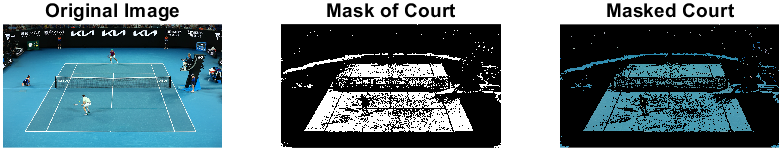
\includegraphics[width=1\textwidth]{SegmentedTennisCourt.png}
    \centering
    \caption{Segmented Tennis Court}
    \label{fig:SegmentedTennisCourt}
\end{figure}